%%%%%%%%%%%%%%%%%%%%%%%%%%%%%%%%%%%%%%%%%
% Programming/Coding Assignment
% LaTeX Template
%
% This template has been downloaded from:
% http://www.latextemplates.com
%
% Original author:
% Ted Pavlic (http://www.tedpavlic.com)
%
% Note:
% The \lipsum[#] commands throughout this template generate dummy text
% to fill the template out. These commands should all be removed when 
% writing assignment content.
%
% This template uses a Perl script as an example snippet of code, most other
% languages are also usable. Configure them in the "CODE INCLUSION 
% CONFIGURATION" section.
%
%%%%%%%%%%%%%%%%%%%%%%%%%%%%%%%%%%%%%%%%%

%----------------------------------------------------------------------------------------
%	PACKAGES AND OTHER DOCUMENT CONFIGURATIONS
%----------------------------------------------------------------------------------------

\documentclass[11pt]{article}

\usepackage{fancyhdr} % Required for custom headers
\usepackage{lastpage} % Required to determine the last page for the footer
\usepackage{extramarks} % Required for headers and footers
\usepackage[usenames,dvipsnames]{color} % Required for custom colors
\usepackage{graphicx} % Required to insert images
\usepackage{listings} % Required for insertion of code
\usepackage{courier} % Required for the courier font
\usepackage{lipsum} % Used for inserting dummy 'Lorem ipsum' text into the template
\usepackage{multirow} %Ligne multiple pour les tableaux
\usepackage[utf8]{inputenc}
\usepackage{indentfirst} %Indentation début de paragraphe

\usepackage{colortbl} %Clouleur tableau protoypes de fonctions


% Margins
\topmargin=-0.45in
\evensidemargin=0in
\oddsidemargin=0in
\textwidth=6.5in
\textheight=9.0in
\headsep=0.25in

\linespread{1.1} % Line spacing

% Set up the header and footer
\pagestyle{fancy}
\lhead{\hmwkAuthorName} % Top left header
\chead{\hmwkClass\ - \hmwkTitle} % Top center head
\rhead{\firstxmark} % Top right header
\lfoot{\lastxmark} % Bottom left footer
\cfoot{} % Bottom center footer
\rfoot{Page\ \thepage\ sur\ \protect\pageref{LastPage}} % Bottom right footer
\renewcommand\headrulewidth{0.4pt} % Size of the header rule
\renewcommand\footrulewidth{0.4pt} % Size of the footer rule

\setlength\parindent{10pt} % Removes all indentation from paragraphs




%----------------------------------------------------------------------------------------
%	NAME AND CLASS SECTION
%----------------------------------------------------------------------------------------

\newcommand{\hmwkTitle}{PROJET JEU} % Titre du document
\newcommand{\hmwkDueDate}{Mercredi 5 février 2014} % Date
\newcommand{\hmwkClass}{CAHIER DES CHARGES } % Type de document
\newcommand{\hmwkClassInstructor}{ } % Teacher/lecturer
\newcommand{\hmwkAuthorName}{Groupe A} % Your name
\newcommand{\hmwkAuthorClasse}{L3 info SPI} % Classe


%----------------------------------------------------------------------------------------
%	TITLE PAGE
%----------------------------------------------------------------------------------------

\title{
\pagenumbering{roman} \setcounter{page}{0} %La page courante sera numérotée en roman et aura l'indice 0 => Pas de numéro car pas de 0 en roman
\vspace{2in}
\textmd{\textbf{\hmwkClass:\ \hmwkTitle}}\\
\normalsize\vspace{0.1in}\small{\hmwkDueDate}\\
\vspace{0.1in}\large{\textit{\hmwkClassInstructor\ }}
\vspace{3in}
}

\author{\textbf{\hmwkAuthorName}}


\date{\hmwkAuthorClasse} % Insert date here if you want it to appear below your name

%----------------------------------------------------------------------------------------

\begin{document}

\thispagestyle{empty}
\maketitle
\newpage


%----------------------------------------------------------------------------------------
%	TABLE OF CONTENTS
%----------------------------------------------------------------------------------------

%\setcounter{tocdepth}{1} % Uncomment this line if you don't want subsections listed in the ToC

\thispagestyle{empty}
\pagenumbering{arabic} \setcounter{page}{0} %Le reste du document est numéroté en arabic à partir de la page 1
\renewcommand\contentsname{Sommaire}
\tableofcontents
\newpage


%----------------------------------------------------------------------------------------
%	Présentation du projet
%----------------------------------------------------------------------------------------

\section{Présentation du projet}

\subsection{Contexte}

Lors du second semestre de troisième année de licence SPI, il est demandé de réaliser un projet. Ce projet à thème imposé n'est autre que le développement d'un logiciel complexe demandant un travail en équipe.\\
Notre équipe de cinq étudiants aura donc du 24 janvier au 16 Mai 2014 pour mettre en œuvre les préceptes de Génie
Logiciel vus au premier semestre afin de présenter un logiciel potentiellement commercialisable par le client, ici représenté par les enseignants.

\subsection{Objectifs}

L'objectif de ce projet est la conception d'une application permettant la création et l'aide à la résolution de puzzles de type picross (henjie).\\
Le joueur pourra commencer des puzzles de différentes tailles ; le but étant de terminer le plus vite possible la partie.


\subsection{Utilisateur cible}

Ce logiciel n'est destiné qu'à un seul joueur à la fois. Cependant, il permet à de nombreux joueurs d'apposer leur
scores à la table des scores.


\subsection{État de l'art}

Les jeux déjà disponibles permettent différentes fonctionnalités :
\begin{itemize}
   \item La création aléatoire et l'édition de grilles de picross de tailles diverses,
   \item La création d'une grille à partir d'une image,
   \item La résolution du puzzle avec ou sans aide à la résolution,
   \item La sauvegarde et le chargement d'une partie,
   \item L'enregistrement et la consultation des scores,
   \item Le partage de ses grilles déjà jouées,
   \item Cocher une case en cliquant dessus une fois, ce qui changera sa couleur,
   \item Marquer un case comme vide en cliquant dessus deux fois et en apposant une croix.
\end{itemize}



%----------------------------------------------------------------------------------------
%	Contraintes initiales
%----------------------------------------------------------------------------------------

\section{Contraintes initiales}


\subsection{Contraintes de jeu}


\begin{itemize}
   \item Le jeu est un picross, le joueur doit noircir les cases en fonction des informations données par les chiffres en
       tête de ligne et de colonne,
   \item Le jeu doit proposer plusieurs tailles de grille (5x5 10x10 15x15 20x20),
   \item L'application doit proposer un éditeur de grille.
\end{itemize}




\subsection{Contraintes de conception}


\begin{itemize}
   \item Le langage de programmation est Ruby/GTK.
   \item Les paramètres de l’application doivent être externalisés afin de pouvoir être modifiés par le joueur (taille
       de la grille).
   \item Le logiciel doit être développé en Programmation Orientée Objet (POO).
   \item Le joueur doit pouvoir sauvegarder une partie pour la reprendre ultérieurement.
\end{itemize}




\subsection{Contraintes temporelles}


\begin{itemize}
    \item Le client impose une réunion hebdomadaire entre les différents acteurs de notre groupe,
    \item Le projet final doit être présenté au client le 16 mai 2014.
\end{itemize}




\subsection{Contraintes matérielles}


\begin{itemize}
    \item Le présent Cahier des Charges doit être remis au client le 16 mai 2014.
    \item Au terme de chaque réunion un compte rendu doit être remis au client.
\end{itemize}


%----------------------------------------------------------------------------------------
%	Spécifications du projet
%----------------------------------------------------------------------------------------


\section{Spécification du projet}

\subsection{Règles détaillées}

\subsubsection{Éléments constituant le jeu}

    \begin{description}
        \item[Grille] : La grille est constituée d'un carré dont le coté est un multiple de 5 cases. Il y a ainsi cinq
            tailles de grilles différentes, 5x5, 10x10, 15x15, et 20x20.
        \item[Case] : Les cases peuvent être noircies, en cliquant dessus à l'aide de la souris. Il est possible de décocher la case en cliquant dessus à nouveau. Il est également possible de cliquer sur une case à l'aide de la souris pour indiquer que la case restera vide, qu'elle ne sera pas noircie.
        \item[Indications extérieures] : Les indications extérieures sont des suites de chiffres sur les bords gauche et supérieur, indiquant le nombre de case à noircir, respectivement dans les lignes et dans les colonnes.
        \item[Chronomètre] : le chronomètre indique le temps qui s'est passé depuis que le joueur a noirci la première case.
    \end{description}

\subsubsection{Principe de fonctionnement du jeu}

\paragraph{But du jeu}
Le but du jeu est de noircir toutes les cases devant être noircies dans le plus court laps de temps possible.

\paragraph{Début d'une partie}

Au début d'une partie, la grille est vierge, et le chronomètre est à 00:00.
\paragraph{Deroulement du jeu.}

Le jeu commence lorsque le joueur noirci un case en cliquant dessus, ce qui enclenche le chronomètre. 

\paragraph{Le menu en cours de partie}

En cours de partie, le joueur peut accéder à un menu spécial où se trouvent~:


\begin{description}
    \item [Sauvegarde de la partie : ]L'utilisateur peut sauvegarder sa partie en cours. Le joueur peut ensuite
        continuer à jouer ou quitter le jeu.~;
   \item [Quitter la partie : ]Renvoie le joueur au menu principal. Il devra avoir pris le soin de sauvegarder ou non sa
       partie.~;
\end{description}


\paragraph{L'interface joueur}

Le joueur noirci des cases ou les rend de nouveau blanches en cliquant dessus à l'aide de la souris. Il peut également cliquer sur un bouton \textbf{Aide} ou sur le bouton \textbf{Menu}.





\subsection{Besoins fonctionnels}

\vspace{0,5cm}
\small
\begin{tabular}{|p{10cm}|p{3cm}|}
	\hline
	\textbf{FONCTIONNALITE} & \textbf{REFERENCE}\\
	\hline
	\hline
		Nouvelle partie 											& F100 \\	\cline{1-2}
		Gérer ses parties											& F110 \\	\cline{1-2}	
		Sauvegarder une partie 										& F111 \\	\cline{1-2}	
		Charger une partie 											& F113 \\	\cline{1-2}	
		Supprimer une partie sauvegardée							& F114 \\	\cline{1-2}	
		Quitter le jeu												& F120 \\	\cline{1-2}	
		Choisir la taille de la grille								& F130 \\	\cline{1-2}
		Fournir une aide 											& F140 \\	\cline{1-2}
		Créer des grilles de jeu									& F150 \\	\cline{1-2}
		Afficher le score											& F160 \\	\cline{1-2}
		Afficher les informations de la grille						& F170 \\	\cline{1-2}
		Afficher le menu du jeu 									& F180 \\	\cline{1-2}
	\hline
	\end{tabular}
\normalsize \\

\begin{itemize}
	\item F100 : Lancer une nouvelle partie
	\item F110 : Le jouer a la possibilité de gerer ses parties à l'aide des fonctionnalitées suivante
	\item F111 : Sauvegarder une partie à n'importe qu'elle moment
	\item F112 : Charger une partie à n'importe qu'elle moment
	\item F114 : Pouvoir supprimer une partie sauvegardée précédement
	\item F120 : Quitter le jeu de n'importe qu'elle endroit
	\item F130 : Choisir la taille de la grille lors d'une nouvelle partie ou de la création de grille
	\item F140 : Mise à disposition d'une aide pour le joueur, de différente degré
	\item F150 : Possibilité de création de grille par le joueur
	\item F160 : Afficher le score du joueur en cours de jeu ou sur le meu principale
	\item F170 : Le joueur a la possibilité de consulter les informations de la grille qui sont disponibles
	\item F180 : Afficher le menu de base du jeu
\end{itemize}

\subsection{Besoins non fonctionnels (optionnels)}

\vspace{0,5cm}
\small
\begin{tabular}{|p{10cm}|p{3cm}|}
	\hline
	\textbf{FONCTIONNALITE} & \textbf{REFERENCE}\\
	\hline
	\hline
		Choisir la langue		 									& F200 \\	\cline{1-2}	
		Affichage de statistiques/classement 						& F210 \\	\cline{1-2}	
		Mise en place d'un fond sonore 								& F220 \\	\cline{1-2}	
		Choix d'un mode de jeu										& F230 \\	\cline{1-2}	
		Création de grille via une image							& F240 \\	\cline{1-2}
	\hline
	\end{tabular}
\normalsize \\

\begin{itemize}
	\item F200 : Le joueur pourra avoir la possibilité de choisir la langue du jeu parmis 
	\item F210 : On pourra consulter les statistiques et classement disponible pour les joueurs ou les grilles proposées
	\item F220 : Mise en place d'un environnement sonore avec possibilité de le désactiver
	\item F230 : Le joueur aura le choix d'un mode de jeu lui proposant un enchainement de partie ainsi qu'une gestion du score différents
	\item F240 : Le joueur aura la possibilité de créer des grilles à partir d'image qu'il importera
\end{itemize}

\newpage
\subsection{Acteur}
	    La figure 1 représente le diagramme du cas d'utilisation avec les différentes fonctionnalitées listées ci-dessus.
	\begin{figure}[!ht]
		\centering
		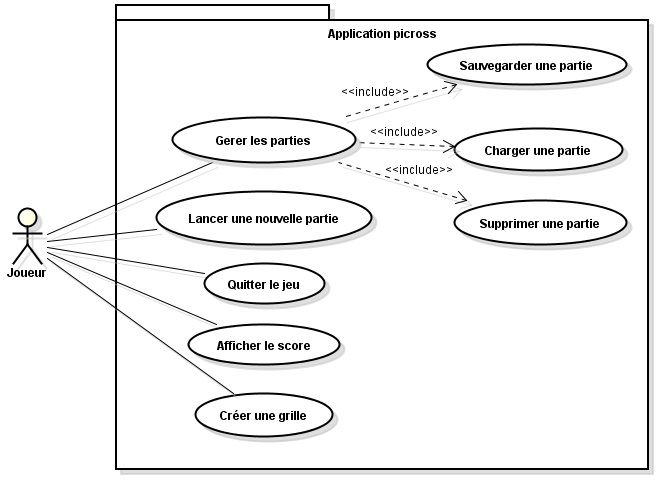
\includegraphics[]{UserCase.jpg}
		\caption{Diagramme du cas d'utilisation}
	\end{figure}
%----------------------------------------------------------------------------------------
%	Déroulement du projet
%----------------------------------------------------------------------------------------

\newpage %pas bien

\section{Déroulement du projet}


\subsection{Livrables}

Les livrables prévus sont :

\begin{itemize}
   \item Le présent cahier des charges validé par le client~;
   \item Dossier de conception~;
   \item Manuel utilisateur~;
   \item Le jeu fonctionnel (livraison le jeudi 16 mai 2014).
\end{itemize}


\subsection{Planning}

Afin de mener à bien ce projet, il est mis à disposition des étudiants 16 séances de 3h (en plus du temps libre) pour permettre aux membres de l'équipe de se retrouver et au chef d'équipe de distribuer les tâches en respectant au mieux le planning mis en place au début du projet.



\subsection{Équipe}

Les membres de l'équipe sont Rémi TREMBLAIN (chef d'équipe), Erwan MARCAHND, Colas PICARD, Kévin CROUILLERE et Anice KHOMANY.





\subsection{Outils de développement}

Voici les différents outils utilisés pour le projet :

\begin{itemize}
   \item Le language de programmation Ruby~;
   \item GTK pour Ruby pour le développement des interfaces graphiques~;
   \item YAML : outil qui permet la sérialisation de données, et qui sera donc utilisé pour la sauvegarde de données, telles que les grilles, les statistiques, la partie en cours~;
   \item GitHub pour la gestion de projet.
\end{itemize}


\subsection{Diagramme WBS}

La figure n°2 représente le diagramme WBS(Struture de découpage du projet), qui correspond à la décomposition hiérarchique du travail que notre équipe doit éxécuter pour remplir les objectifs et produire les livrables voulus en respectant les délais.
	
\begin{figure}[!ht]
		\centering
		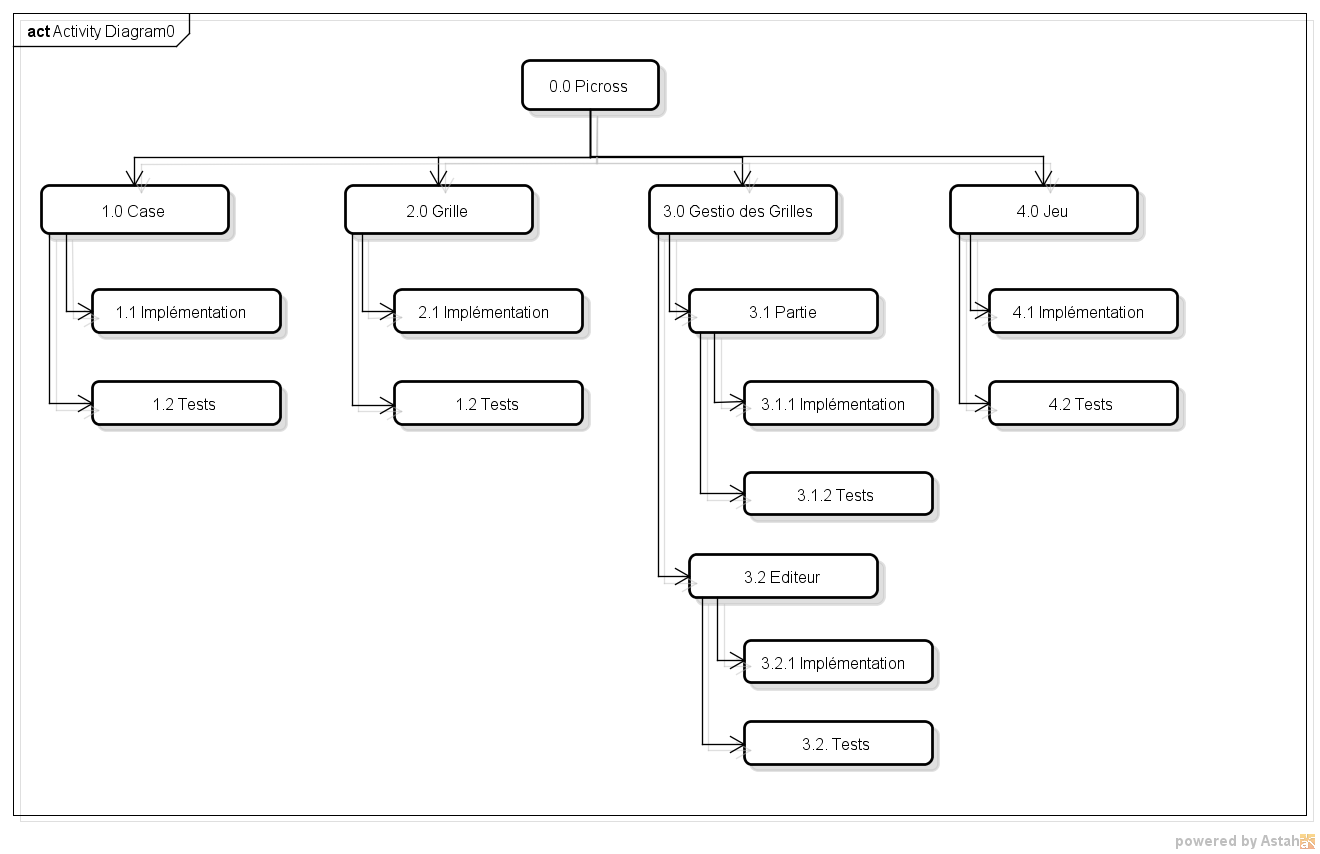
\includegraphics[]{WBS.png}
		\caption{Diagramme WBS}
	\end{figure}

    \subsection{Diagramme de Gantt}
    Il s'agit d'une représentation graphique de l'avancement temporel du projet, visible sur la figure n°3.
    
    \begin{tabular}{}
	    \hline
    	\textbf{N°} & \textbf{nom} & \textbf{Durée} & \textbf{Date de Début} & \textbf{Date de Fin} & \textbf{Prédecesseur}\\\
    	\hline
        \hline
    		1 & Rédaction du Cahier des charges & 26 Jours & 24/01/2014 & 28/02/2014 \\ \cline{1-2}
    		2 & Rédaction du Dossier de Conception & 7 jours & 03/03/2014 & 11/03/2014 & 1  \\	\cline{1-2}	
        	3 & Developpement des fonctions principales & 30 jours & 12/03/2014 & 22/04/2014 & 2 \\	\cline{1-2}	
    		4 & Rédaction du Manuel utilisateur & 30 jours & 12/03/2014 & 22/04/2014 & 2    \\	\cline{1-2}	
    		5 & Test des fonctions principales & 2 jours & 23/04/2014 & 24/04/2014 & 3  \\	\cline{1-2}
            6 & Correction des erreurs & 2 jours & 25/04/2014 & 28/04/2014 & 5 \\ \cline{1-2}
            7 & Developpement des fonctions optionnelles & 7 jours & 29/04/2014 & 7/05/2014 & 6 \\ \cline{1-2}
            8 & Test des fonctions optionnelles & 2 jours & 08/05/2014 & 9/05/2014 & 7 \\ \cline{1-2}
            9 & Correction des erreurs & 2 jours & 12/05/2014 & 13/05/2014 & 8 \\ \cline{1-2}
           10 & Relecture du Projet & 2 jours & 14/05/2014 & 15/05/2014 & 6, 9 \\ \cline{1-2}
           11 & Remise du Produit & 1 jour & 16/05/2014 & 16/05/2014 & 6, 9 \\ \cline{1-2}
    	\hline
	\end{tabular}



%----------------------------------------------------------------------------------------
%	Gloassaire
%----------------------------------------------------------------------------------------

\section{Glossaire}

\begin{description}
\item [GTK : ]Gimp ToolKit
\item [POO : ]Programmation Orientée Objet
\item [YAML : ]YAML ain't markup language (acronyme récursif)
\end{description}

\renewcommand{\thefootnote}{\*} %Ne pas numéroter la note de bas de page
\footnotetext{Note : Les chiffres et pourcentages sont fournis à titre indicatif. Il pourront être modifiés pour une meilleure jouabilité.}



\end{document}
